% !TEX root = ../thesis.tex

\begin{figure}[t!]
	\centering
	\subfigure[Logistic sigmoid.]{
    		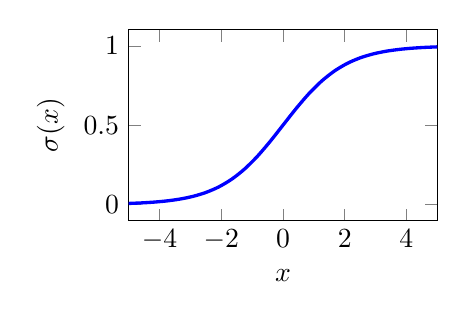
\begin{tikzpicture}
			\begin{axis}[width=5.5cm,height=4cm,ylabel=$\sigma(x)$,xlabel=$x$,ymin=-0.1,ymax=1.1,xmin=-5,xmax=5]
				\addplot[very thick,blue,smooth] {1/(1+exp(-x))};
			\end{axis}
		\end{tikzpicture}
	}
	\subfigure[Hyperbolic tangent.]{
		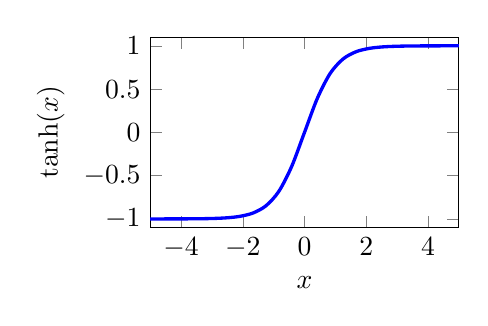
\begin{tikzpicture}
			\begin{axis}[width=5.5cm,height=4cm,ylabel=$\tanh(x)$,xlabel=$x$,ymin=-1.1,ymax=1.1,xmin=-5,xmax=5]
				\addplot[very thick,blue,smooth] {tanh(x)};
			\end{axis}
		\end{tikzpicture}
	}\\
	\subfigure[Rectifier linear unit \cite{Nair2010}.]{
    		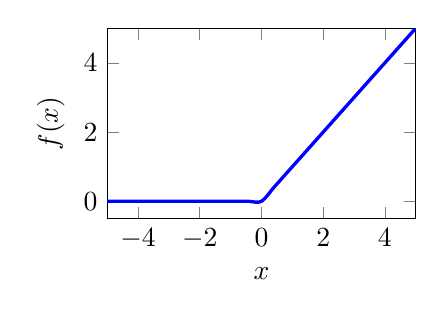
\begin{tikzpicture}
			\begin{axis}[width=5.5cm,height=4cm,ylabel=$f(x)$,xlabel=$x$,ymin=-0.5,ymax=5,xmin=-5,xmax=5]
				\addplot[very thick,blue,smooth] {max(0, x)};
			\end{axis}
		\end{tikzpicture}
	}
	\subfigure[Identity function.]{
		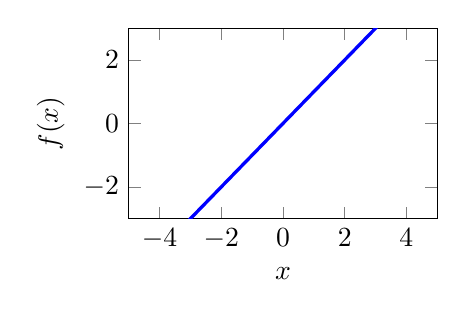
\begin{tikzpicture}
			\begin{axis}[width=5.5cm,height=4cm,ylabel=$f(x)$,xlabel=$x$,ymin=-3,ymax=3,xmin=-5,xmax=5]
				\addplot[very thick,blue,smooth] {x};
			\end{axis}
		\end{tikzpicture}
	}
    	\caption[Sigmoidal activation functions.]{Common choise of activation functions includes logistic sigmoid $\sigma(z)$ and hyperbolic tangent $tanh(z)$. Convolutional neural networks often rely on ReLU and identity functions.}
    	\label{fig:act}
\end{figure}
